\documentclass{article}
\usepackage{fullpage}
\usepackage{graphicx}

\title{16.35 PSet \#1}
\author{Ryan Fish}
\date{\today}

\begin{document}
\maketitle

\section*{Pre-deliverables}
\section{Real-time Systems and Software}
\begin{itemize}
\item Learn the language of software requirements so I can communicate them to a design team, and interpret needs from conversations with customers.
\item Be exposed to common errors made in this field so I may learn by example rather than experience.  Life-critical systems aren't a good place for learning by experience.
\item Practice building real-time software and systems to prepare for a hopeful career in embedded mechanical control systems.
\end{itemize}
\section{Documentation}
\subsection{Java version on Athena}
\begin{enumerate}
	\item 1.7.0\_65
	\item ran \verb! java -version ! on an athena remote session
	\item Googled \verb| check java version linux | and logged in to athena remotely, maybe 45 seconds all told
\end{enumerate}


\subsection{Enable assertions}
\begin{enumerate}
	\item  Assertions in the program are enabled by running java with the \verb| -ea | flag
	\item http://docs.oracle.com/javase/8/docs/technotes/guides/language/assert.html\#enable-disable
	\item 20 seconds via Google
\end{enumerate}

\subsection{Double to string}
\begin{enumerate}
	\item \verb|String doub = Double.toString(num) | where \verb| num | is the input double and \verb| doub | is the output String
	\item http://docs.oracle.com/javase/7/docs/api/java/lang/Double.html
	\item found via google, 2 minutes to verify it produces the expected output
\end{enumerate}

\subsection{Create jar with files from dir \tt asst1}
\begin{enumerate}
	\item \verb|jar cf asst1.jar asst1|
	\item http://docs.oracle.com/javase/tutorial/deployment/jar/build.html
	\item 20 seconds via Google
\end{enumerate}

\setcounter{section}{3}
\section{Reqs and Unit Testing}
\subsection{Faults in Assignment requirements}
\begin{enumerate}
	\item No outline of variables or state that gets referenced in method description
	\item Requirements are not numbered, harder to trace to tests
	\item Requirements are not always written in a specifically testable manner, and use should poorly
\end{enumerate}
\subsection{Specific failings}
\begin{enumerate}
	\item The specification of the output of the program is a should statement, something like output format needs to be determined with a shall statement.
	\item The simulator class clock is not well defined in terms of purpose or format.
	\item No description is given for how to deal with failure to provide valid inputs e.g. to the GroundVehicle constructor.
\end{enumerate}
\subsection{GroundVehicle reqs}
TODO
\subsection{List of Unit Tests}
\subsubsection{Test needed}
\begin{enumerate}
	\item my util.clampDouble method
	\item my util.clampInt method
	\item my util.wrapAngle method
	\item Control constructor
	\item controlVehicle
	\item getVelocity
	\item setVelocity
	\item updateState
	\item getControl
	\item setNumSides
	\item main
\end{enumerate}
\subsubsection{No Tests needed}
\begin{enumerate}
	\item getSpeed - simple getter
	\item getRotVel - simple getter
	\item getPosition - simple getter
	\item getCurrentSec - simple getter
	\item getCurrentMSec - simple getter
	\item setPosition - relies on clamp and wrap 
	\item GroundVehicle constructor - relies on setPosition and controlVehicle
	\item run
\end{enumerate}
\subsubsection{Equivalence Classes}
\begin{enumerate}
	\item First arg greater than bounds, less than bounds, within bounds, again for second arg
	\item 
\end{enumerate}

\section{Output}
\begin{figure}
\centering
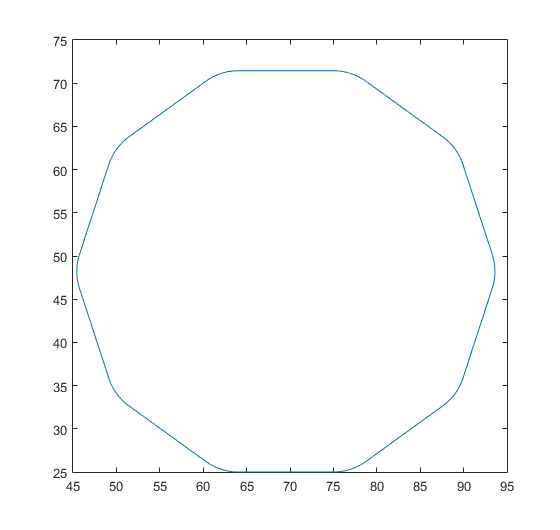
\includegraphics[width=0.7\linewidth]{10}
\caption[Decagon]{Decagon}
\end{figure}
\begin{figure}
\centering
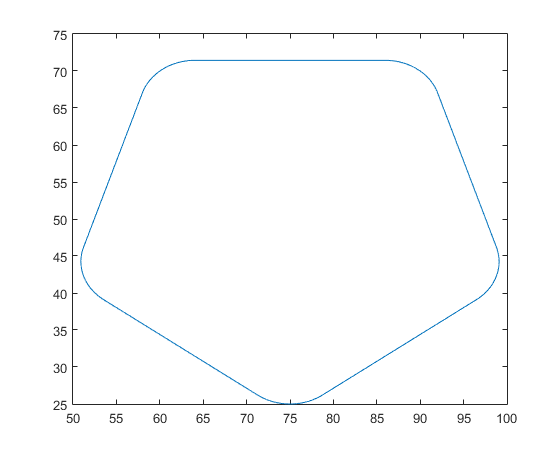
\includegraphics[width=0.7\linewidth]{5}
\caption[Pentagon]{Pentagon}
\end{figure}
\section{Code control}
\subsection{Subversion Log}
\begin{enumerate}
	\item
	\begin{verbatim}
	$ git commit -am "oops, now I have read section 6, and rearranged files properly"
	[master 6064bee] oops, now I have read section 6, and rearranged files properly
	11 files changed, 249 insertions(+), 14 deletions(-)
	rename asst1/{src => }/Control.java (100%)
	rename asst1/{src => }/GroundVehicle.java (100%)
	rename asst1/{src => }/Simulator.java (100%)
	rename asst1/{src => }/util.java (100%)
	\end{verbatim}
	\item maybe 6 hours on the code and 30 seconds on the file copying and committing.
\end{enumerate}


\end{document}